\documentclass[12pt,letterpaper]{exam}

\newcommand{\DocTitle}{Renew the DocTitle variable.}
\newcommand{\CourseNumber}{NE555}
\newcommand{\CourseName}{Nuclear Reactor Dynamics}
\newcommand{\DayTime}{TuTh 8:00-9:15}
\newcommand{\Room}{VV\&E B129}
\newcommand{\Term}{Spring 2011}
\newcommand{\Instructor}{Lewis John Lloyd}
\newcommand{\School}{University of Wisconsin - Madison}

\usepackage{listings}
\usepackage{mathtools}
\usepackage{xtab}
\usepackage{longtable}
\usepackage{array}
\usepackage{mathrsfs}
\usepackage{color}
\usepackage{multicol}
\usepackage{pdflscape}
\usepackage{pdfpages}
\usepackage{graphicx}
\usepackage{esint}
\usepackage{amsmath}
\usepackage{amssymb}
\usepackage{graphics}

\usepackage[
			pdfborder={0 0 0},
			urlcolor=cyan,
			pdftitle={\CourseNumber \DocTitle},
			pdfauthor={\Instructor}
			]{hyperref}
			
\usepackage[
			includeheadfoot,
			top=0.5in,
			bottom=0.5in,
			left=1.0in,
			right=1.0in
			]{geometry}
\setlength{\parindent}{0in}
\setlength{\parskip}{\baselineskip}

\lhead{\CourseNumber: \CourseName}
\chead{}
\rhead{\Term}
\lfoot{}
\cfoot{\thepage}
\rfoot{}
\coverlhead{\CourseNumber: \CourseName}
\coverchead{}
\coverrhead{\Term}
\coverlfoot{}
\covercfoot{\School}
\coverrfoot{}


\correctchoiceemphasis{\bfseries\color{red}}
\bracketedpoints
\pointsinmargin
%\addpoints
%\shadedsolutions

\lstset{ %
language=Matlab,                % the language of the code
basicstyle=\footnotesize,       % the size of the fonts that are used for the code
numbers=left,                   % where to put the line-numbers
numberstyle=\footnotesize,      % the size of the fonts that are used for the line-numbers
stepnumber=5,                   % the step between two line-numbers. If it's 1, each line 
                                % will be numbered
numbersep=5pt,                  % how far the line-numbers are from the code
backgroundcolor=\color{white},  % choose the background color. You must add \usepackage{color}
showspaces=false,               % show spaces adding particular underscores
showstringspaces=false,         % underline spaces within strings
showtabs=false,                 % show tabs within strings adding particular underscores
frame=single,                   % adds a frame around the code
tabsize=2,                      % sets default tabsize to 2 spaces
}

\renewcommand{\solutiontitle}{\noindent\textbf{Solution:}\par\noindent}

\newcommand{\mathsym}[1]{{}}
\newcommand{\unicode}{{}}
\newcommand{\tr}[1]{\tilde{#1}}
\newcommand{\LapTran}[1]{\mathscr{L}\left[#1\right]}
\newcommand{\InvLapTran}[1]{\mathscr{L}^{-1}\left[#1\right]}
\newcommand{\ParDer}[2]{\frac{\partial #1}{\partial #2}}
\newcommand{\Der}[2]{\frac{d\; #1}{d\;#2}}


\renewcommand{\DocTitle}{Problem Set 01}
\noprintanswers

%-------------------------------------------------------------------------------------
\begin{document}
%-------------------------------------------------------------------------------------
\begin{center}
\textbf{\DocTitle}
\end{center}
%-------------------------------------------------------------------------------------

\begin{questions}
\question[10]{
Write down a differential equation for the time-dependent, continuous-energy, neutron diffusion equation in a multiplying media, without a source term.
Describe what each term represents.
\fullwidth{\begin{solution}
$\underbrace{\frac{1}{v}\frac{\partial \phi}{\partial t}}_{1} = 
-\underbrace{\nabla\cdot(-D\nabla\phi)}_{2} 
-\underbrace{\Sigma_t\phi}_{3} 
+ \underbrace{\int\limits_0^{\infty}\Sigma_s(E'\rightarrow E)\phi(E')dE'}_{4}
+\underbrace{\chi(E)\int\limits_0^{\infty}\nu(E')\Sigma_f(E')\phi(E')dE'}_{5}$
\begin{enumerate}
\item{$\displaystyle\frac{1}{v}\frac{\partial \phi}{\partial t}$
represents the time rate of change of the total number of neutrons.
}
\item{$\displaystyle-\nabla\cdot(-D\nabla\phi)$
represents the divergence of the neutron current within a control volume.
}
\item{$\displaystyle-\Sigma_t\phi$
represents the rate at neutrons are removed from one particular energy via all possible interactions with other particles within a control volume.
}
\item{$\displaystyle\int\limits_0^{\infty}\Sigma_s(E'\rightarrow E)\phi(E')dE'$
represents the rate at which neutrons are scattered into one particular energy from all other energies within a control volume.
}
\item{$\displaystyle\chi(E)\int\limits_0^{\infty}\nu(E')\Sigma_f(E')\phi(E')dE'$
represents the rate at which neutrons of a given energy are being produced through fission within the control volume.
}
\end{enumerate}
\end{solution}}}
\ifprintanswers
\pagebreak
\fi
\question[15]{
Evaluate the following complex integral by integrating over the left half of the complex plane. $\gamma$ is an arbitrary constant that ensures that all singularities are within the integration contour. $a$ and $b$ are positive, arbitrary, real constants.

$$I = \frac{1}{2\pi\mathrm{i}}\int\limits_{\gamma-\mathrm{i} \infty}^{\gamma+\mathrm{i}\infty}\frac{e^{s\,t}}{(s+a)(s+b)}ds$$

HINT: It will be easier to use a change of variable to recenter the complex plane around $\gamma$, such as $s = \gamma + \mathrm{i}\omega$.

\fullwidth{\begin{solution}
To evaluate the integral, recognize that it is the inverse of the Laplace Transform.
While you can use a table and partial fraction expansions, you can instead evaluate this integral directly. 
$$I = \frac{1}{2\pi\mathrm{i}}\int\limits_{\gamma-\mathrm{i} \infty}^{\gamma+\mathrm{i}\infty}\frac{e^{s\,t}}{(s+a)(s+b)}ds$$
This integral can be evaluated with an application of the Residue Theorem and Jordan's Lemma.
To properly evaluate the integral, you must use a contour that encompasses all of the singularities on the left half of the complex plane.
The contour should be a semicircle; this is where Jordan's Lemma comes into play.
By using the change of variable hinted at in the problem, you get to the following:

$$\frac{1}{2\pi\mathrm{i}}\int\limits_{\gamma-\mathrm{i} \infty}^{\gamma+\mathrm{i}\infty}\frac{e^{s\,t}}{(s+a)(s+b)}ds = \sum_{k=1}^{n} Res(f,z^k)+\frac{e^{\gamma}}{2\,\pi}\varointctrclockwise_{-\infty}^{\infty}\frac{e^{\mathrm{i}\,\omega\,t}}{(\omega-\mathrm{i}(a+\gamma))(\omega-\mathrm{i}(b+\gamma))}\; d\omega$$

The contour integral on the right is equal to zero by Jordan's Lemma.
This means that the total integral evaluates to:
$$I = \frac{e^{-a\,t}-e^{-b\,t}}{b-a}$$

 

\end{solution}}}
\ifprintanswers
\pagebreak
\fi

\question[15]{
A one-dimensional slab reactor consists of two regions: a multiplying core of length $a$, and vacuum outside of the core.
Using one-group diffusion theory, determine $a$ such that the reactor will be critical.
Express $a$ in terms of relevant nuclear properties.

\fullwidth{\begin{solution}

For a critical, one-dimensional reactor, the steady-state neutron balance is give by:

$$\displaystyle D \nabla^2\phi-\Sigma_a\phi =  -\nu\Sigma_f\phi$$
A critical reactor can be expressed in terms of the lowest eigenvalue representation of the Helmholtz Equation:$$\displaystyle\nabla^2\phi+B_g^2\phi = 0$$
$B_g^2$ is the geometric buckling term, which, for a slab, is given as $\displaystyle\left(\frac{\pi}{\tilde{a}}\right)^2$.

Using some algebra, $$\displaystyle \frac{\nabla^2\phi}{\phi} = \frac{\Sigma_a-\nu\Sigma_f}{D}  = -B_g^2$$
\begin{eqnarray*}
-B_g^2 & = &\frac{\Sigma_a-\nu\Sigma_f}{D}\\
\left(\frac{\pi}{\tilde{a}}\right)^2 & = &\frac{\nu\Sigma_f-\Sigma_a}{D}\\
\frac{\pi}{\tilde{a}} & = &\sqrt{\frac{\nu\Sigma_f-\Sigma_a}{D}}\\
\tilde{a} & = & \frac{\pi\, \sqrt{D}}{\sqrt{\nu\Sigma_f-\Sigma_a}}\\
a + 2 z_o & = & \frac{\pi\, \sqrt{D}}{\sqrt{\nu\Sigma_f-\Sigma_a}}
\end{eqnarray*}

Here, $z_o$ is given by:
$$\displaystyle z_o = 0.7123\lambda_{tr} \simeq 2.1\,D$$

Giving for a final solution:
$$ a \simeq \frac{\pi\, \sqrt{D}}{\sqrt{\nu\Sigma_f-\Sigma_a}} - 4.2\,D$$
\end{solution}}}
\ifprintanswers
\pagebreak
\fi
\question[15]{
Use a computer to plot the solution to the following coupled ODEs.
Plot $y(t)$ and $x(t)$ on the same graph for $t \in [0,10]$.

\begin{minipage}{0.4\linewidth}\begin{eqnarray*}
\frac{dy}{dt} & = & 0.4\, x(t) - y(t) \\
\frac{dx}{dt} & = & -0.4\, y(t)
\end{eqnarray*}\end{minipage}
,
\begin{minipage}{0.4\linewidth}\begin{eqnarray*}
y(0) & = & 1 \\
x(0) & = & 0
\end{eqnarray*}\end{minipage}
\fullwidth{\begin{solution}
First, obtain an analytic solution to the system.
Do not fret; this is not required for points.
\begin{multicols}{2}
Laplace Transform both equations.
\begin{eqnarray*}
\LapTran{\frac{dy}{dt}} & = & 0.4\,\LapTran{x}-\LapTran{y}\\
\LapTran{\frac{dx}{dt}} & = & -0.4\,\LapTran{y}\\
s\,\tr{y} - 1 & = & 0.4\,\tr{x}-\,\tr{y}\\
s\,\tr{x} & = & -0.4\,\tr{y}\\
\end{eqnarray*}
Solve for $\tr{x}$ in terms of $\tr{y}$.
\begin{eqnarray*}
s\,\tr{x} & = & -0.4\,\tr{y}\\
\tr{x} & = & -0.4\frac{\tr{f}}{s}\\
\end{eqnarray*}
Eliminate $\tr{x}$ from the equation for $\tr{y}$ and solve for $\tr{x}$.
\begin{eqnarray*}
s\,\tr{y} +\tr{y} + 0.16\,\frac{\tr{y}}{s}& = & 1\\
\tr{y}\left(s+1+\frac{0.16}{s}\right) & = & 1\\
\tr{y}\left(\frac{s^2+s+0.16}{s}\right) & = & 1\\
\end{eqnarray*}
\begin{eqnarray*}
\tr{y} & = & \frac{s}{s^2+s+0.16}\\
\tr{y} & = & \frac{s}{(s+0.8)(s+0.2)}\\
\end{eqnarray*}
Apply the Inverse Laplace Transform.
\begin{eqnarray*}
y(t) & = & \InvLapTran{\frac{s}{(s+0.8)(s+0.2)}}\\
y(t) & = & \frac{4}{3}e^{-0.8\,t}-\frac{1}{3}e^{-0.2\,t}\\
\end{eqnarray*}

Integrating $y(t)$ with respect to $t$ will yield $x(t)$.

$$x(t) = \frac{2}{3}\left(e^{-0.8\,t}-e^{-0.2\,t}\right)$$

Giving the final solutions of 
\begin{eqnarray*}
y(t) & = & \frac{4}{3}e^{-0.8\,t}-\frac{1}{3}e^{-0.2\,t}\\
x(t) & = & \frac{2}{3}\left(e^{-0.8\,t}-e^{-0.2\,t}\right)\\
\end{eqnarray*}
See next page for graph.

\end{multicols}
\vfill


\end{solution}}}
\end{questions}
\ifprintanswers
\begin{landscape}
%\pagestyle{empty}
%\begin{figure*}
%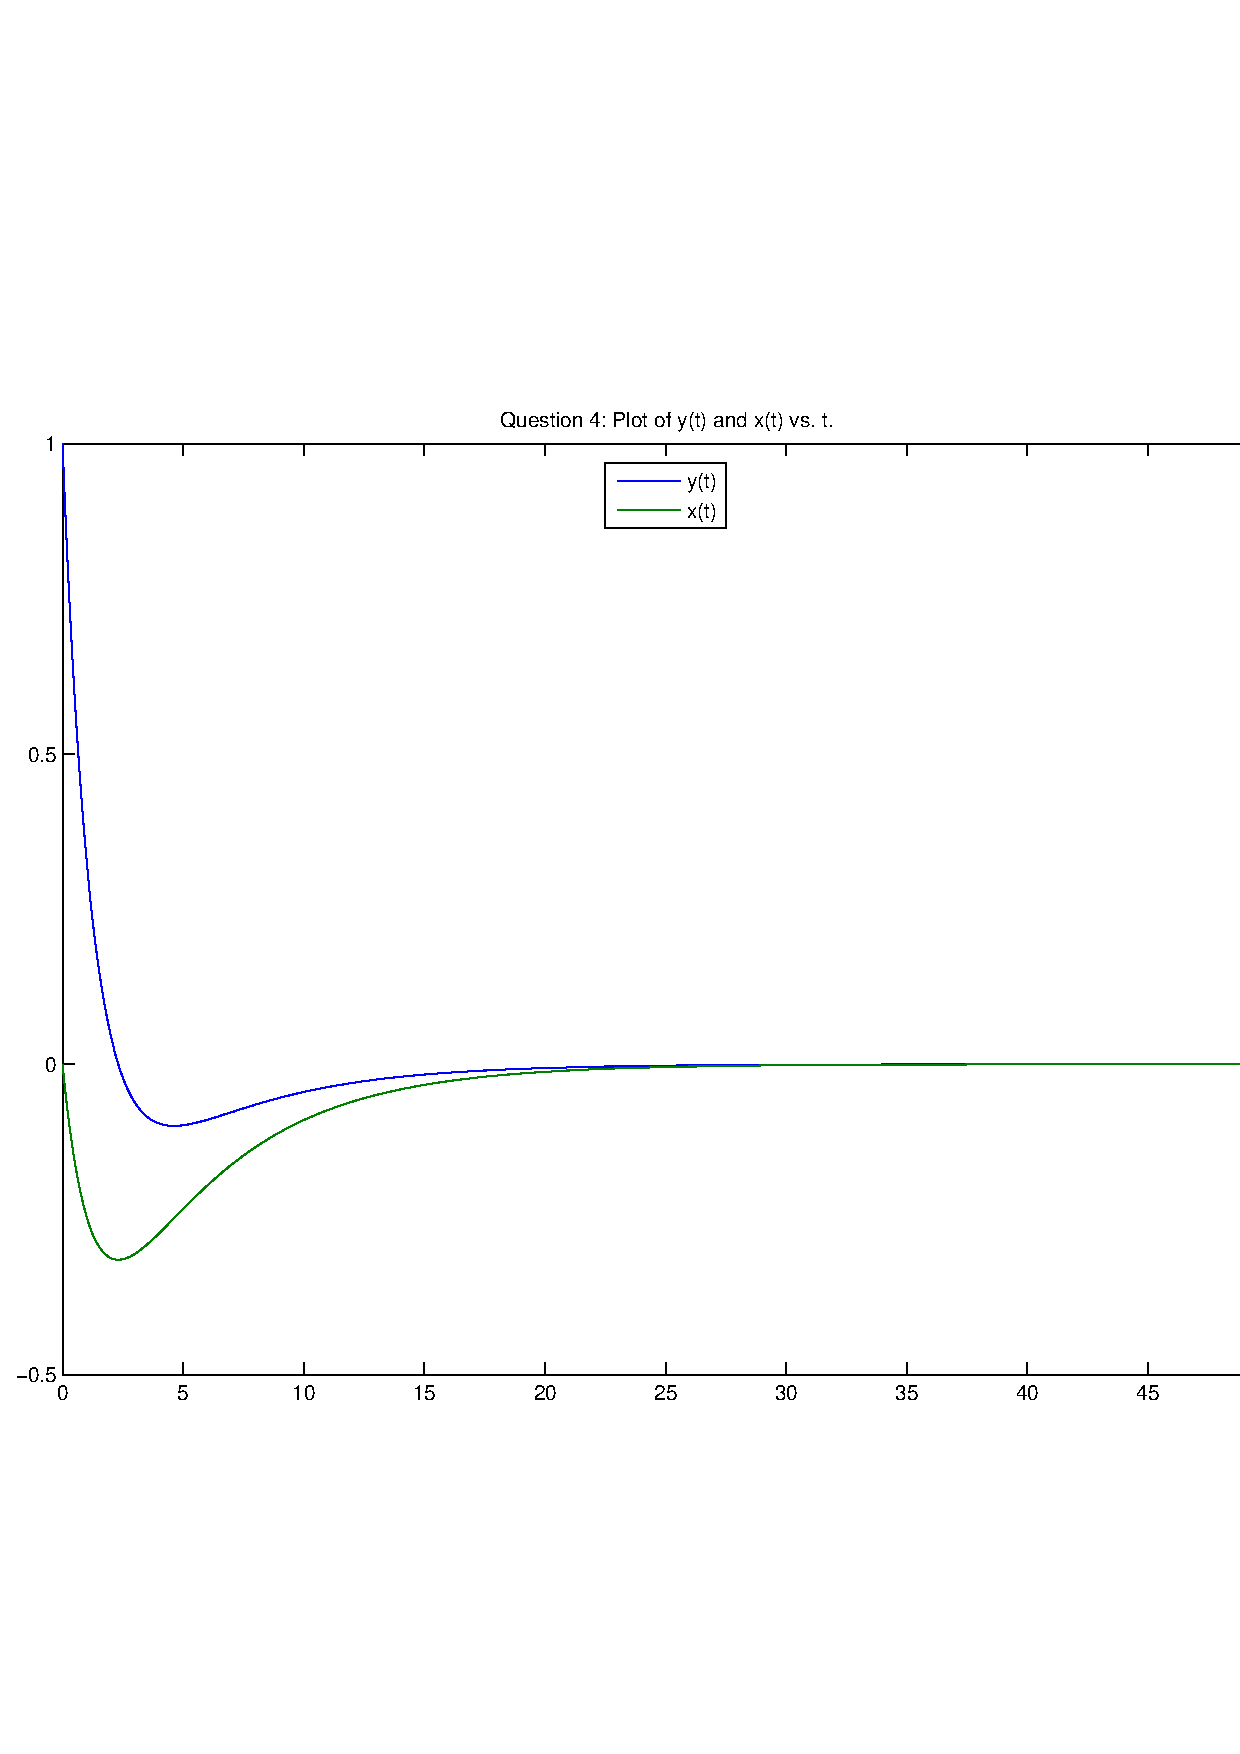
\includegraphics[angle=0,scale=0.95]{PS01Q04pic.pdf}
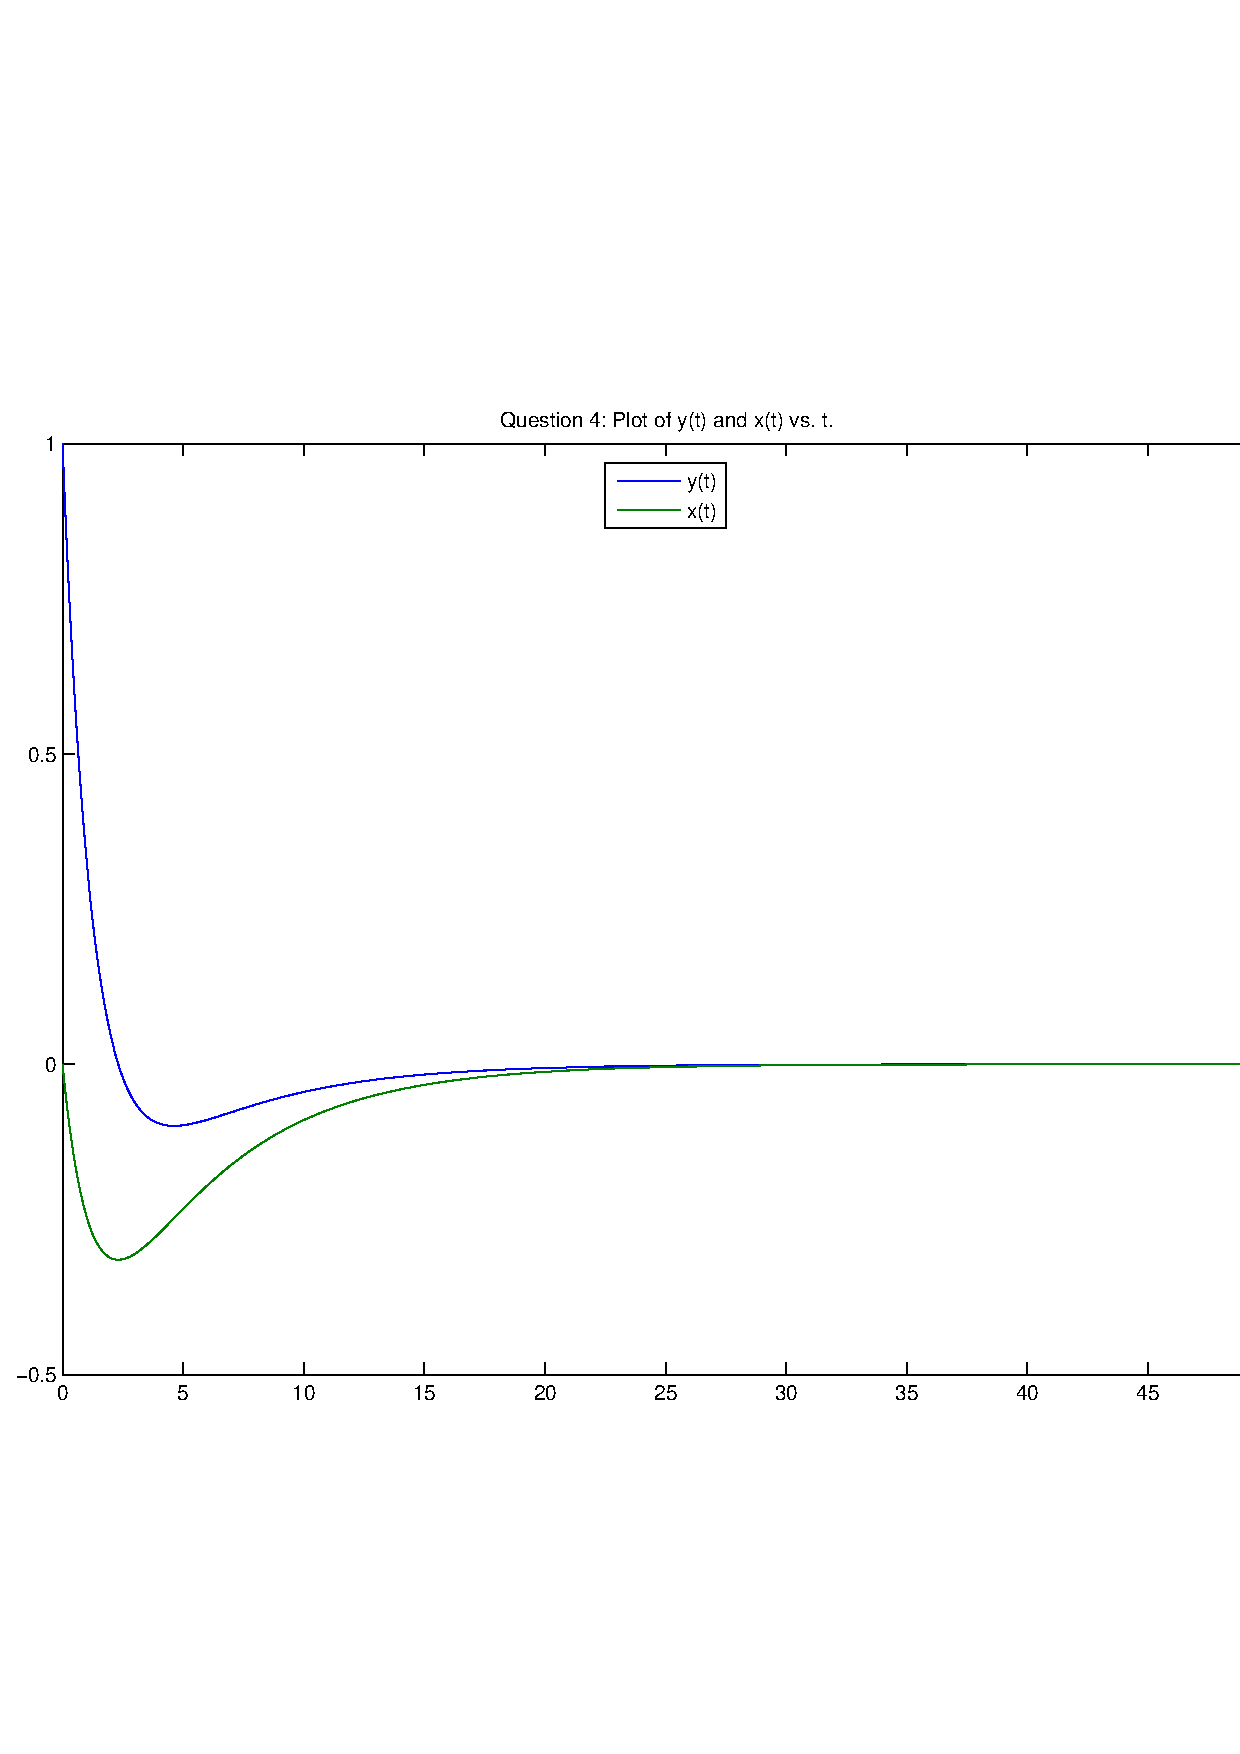
\includepdf[landscape=true]{PS01Q04pic.pdf}
%\end{figure*}
\end{landscape}

\fi
\end{document}